% \section{Atividades}
%
% Neste módulo, foram realizadas atividades práticas voltadas à análise e
% manipulação de metadados em arquivos digitais, exploração de estruturas
% forenses de sistemas de arquivos e aquisição de imagem de disco em ambiente
% \textit{Kali Linux}.
%
% As atividades envolveram a leitura, remoção e escrita de metadados com a
% ferramenta \textit{ExifTool}, análise de inodes e estruturas de partição com o
% \textit{The Sleuth Kit (TSK)}, além da criação de cópia bit a bit de partição
% com o utilitário \textit{dd}, permitindo compreender procedimentos básicos de
% forense computacional.
%
% Cada atividade apresenta abaixo o respectivo print solicitado, acompanhado de
% descrição explicativa conforme exigido nas orientações do módulo.
%
% \newpage
%
\question[Atividade 12.6]{Ler metadados no Kali Linux}

\begin{figure}[H]
\centering
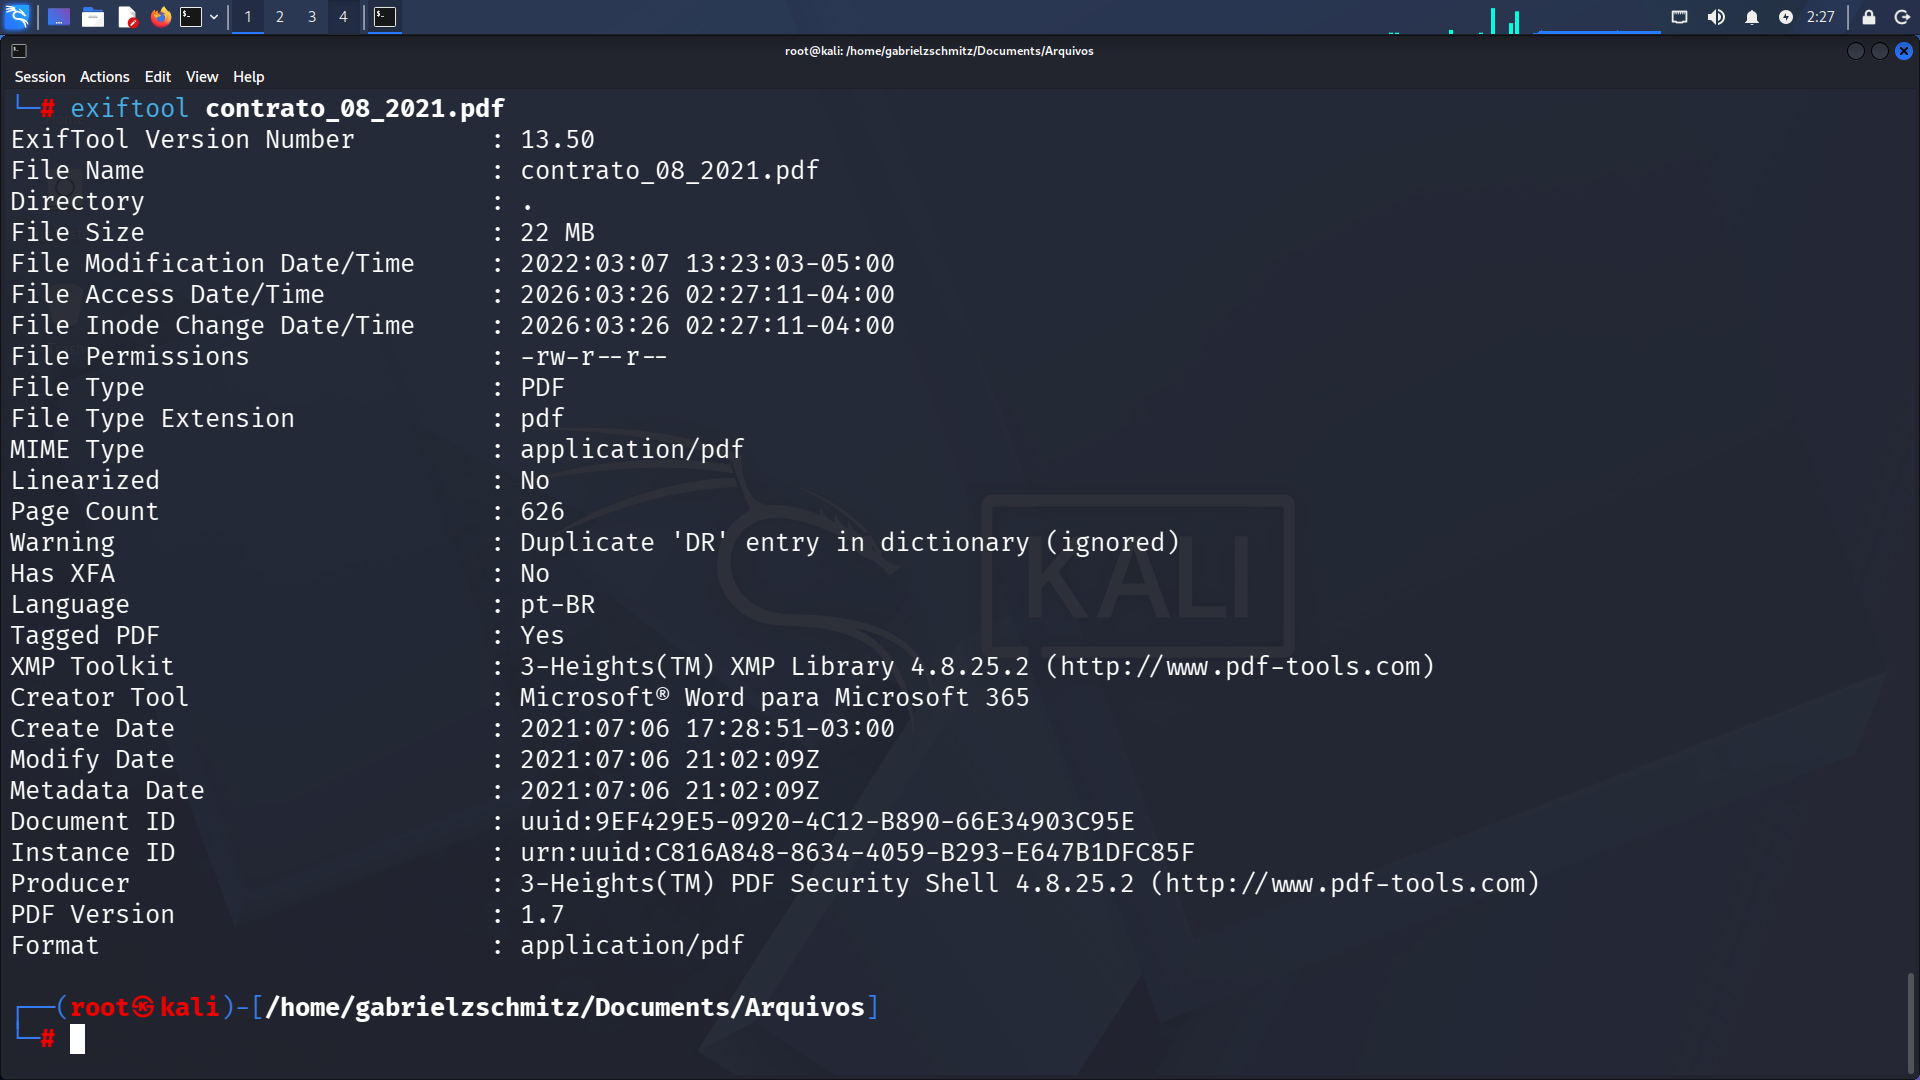
\includegraphics[width=0.99\textwidth]{./fig/fig12.6.png}
\caption{Leitura dos metadados do arquivo contrato\_08\_2021.pdf com exiftool}
\label{fig:fig12.6}
\end{figure}

\newpage

\question[Atividade 12.7]{Apagando metadados no Kali Linux}

\begin{figure}[H]
\centering
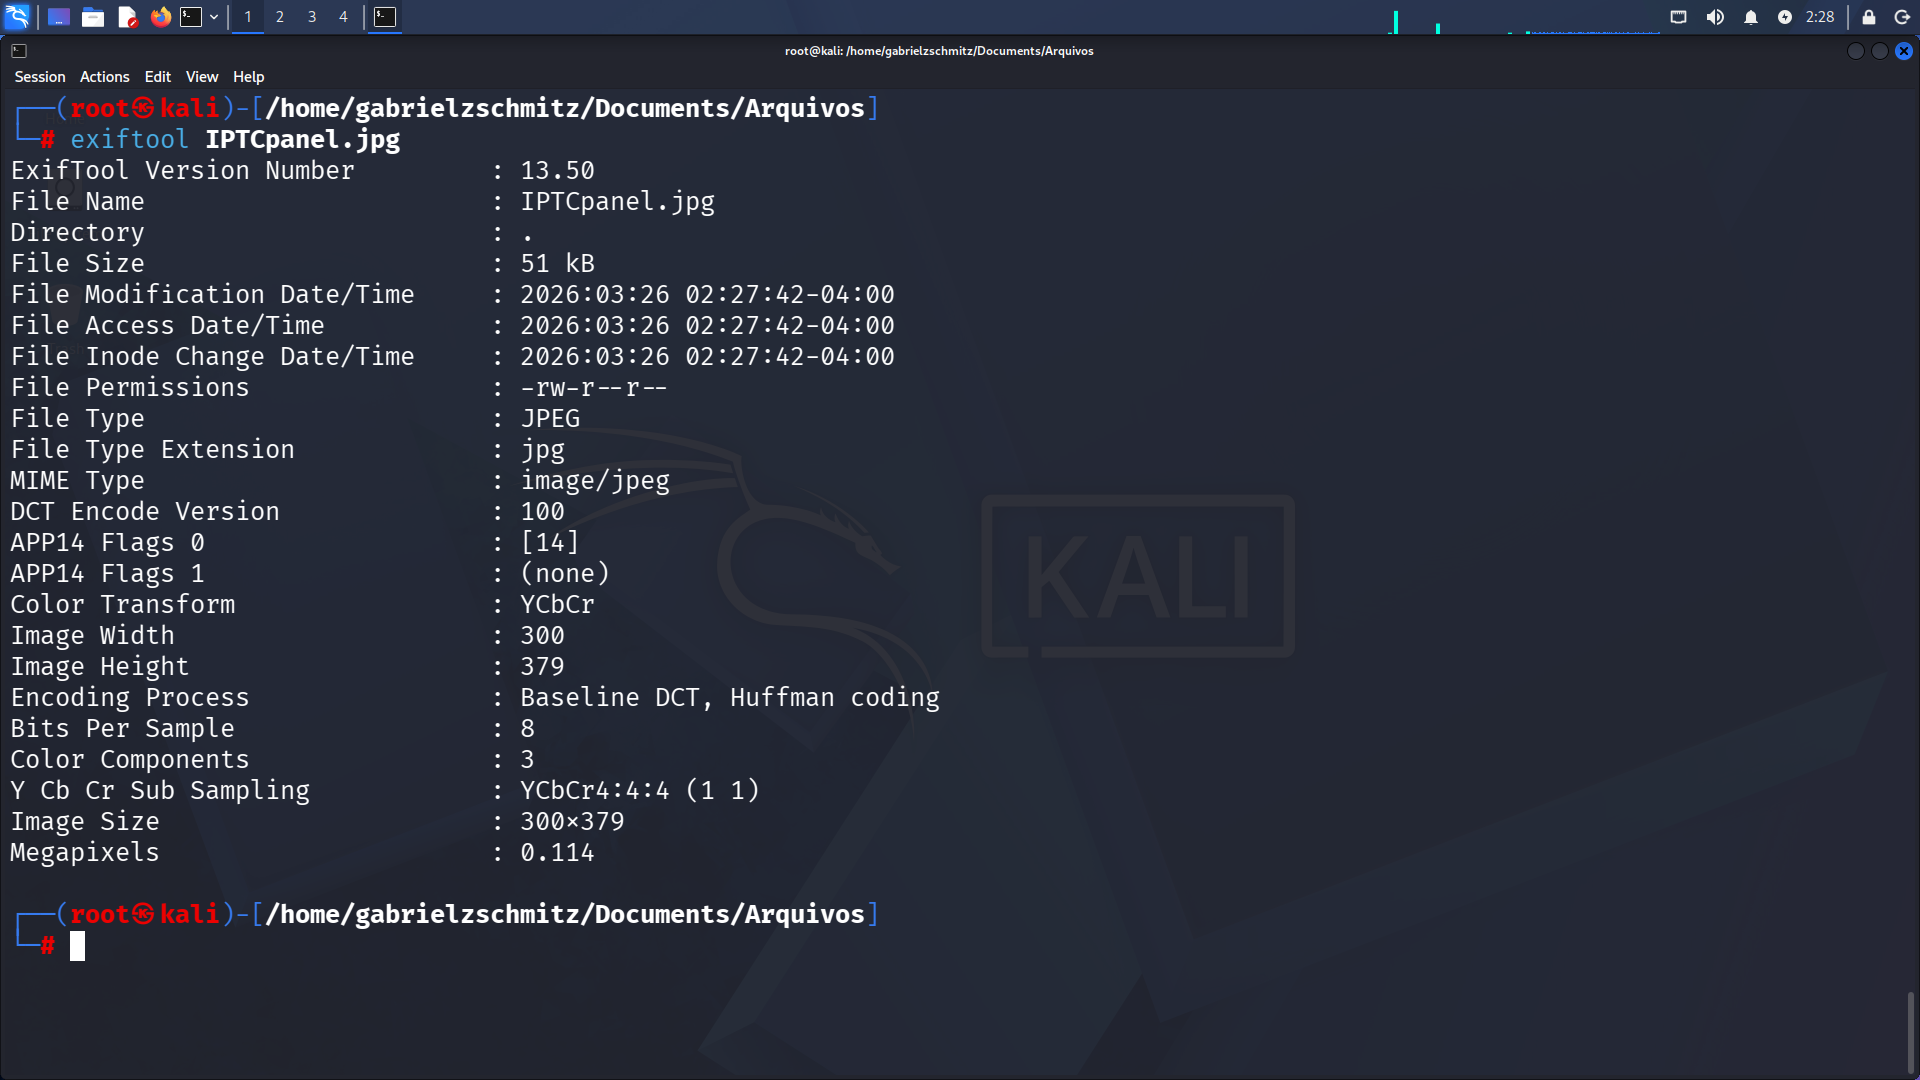
\includegraphics[width=0.99\textwidth]{./fig/fig12.7.png}
\caption{Arquivo IPTCpanel.jpg após remoção dos metadados}
\label{fig:fig12.7}
\end{figure}

\newpage

\question[Atividade 12.8]{Escrevendo metadados no Kali Linux}

\begin{figure}[H]
\centering
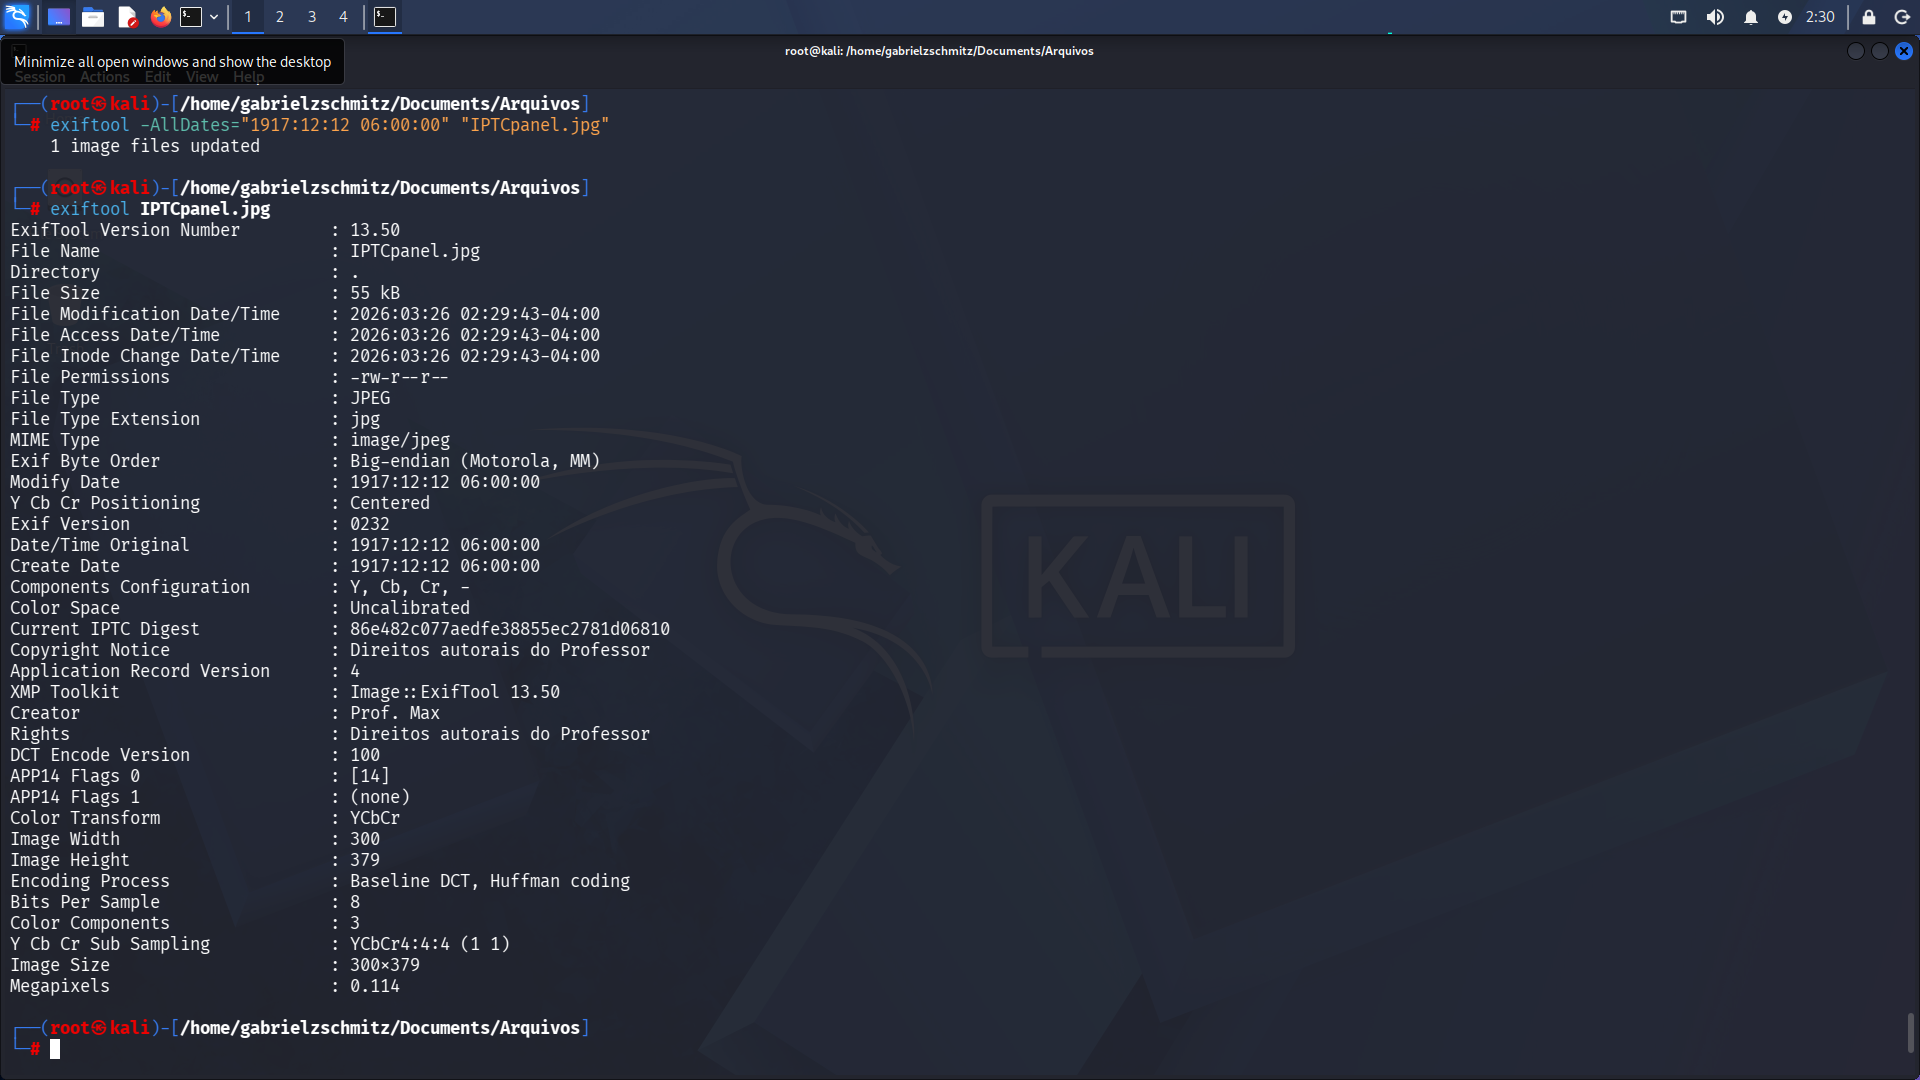
\includegraphics[width=0.99\textwidth]{./fig/fig12.8.png}
\caption{Metadados atualizados no arquivo IPTCpanel.jpg após escrita com exiftool}
\label{fig:fig12.8}
\end{figure}

\newpage

\question[Atividade 12.9]{Explorando The Sleuth Kit (TSK) no Kali Linux}

\begin{figure}[H]
\centering
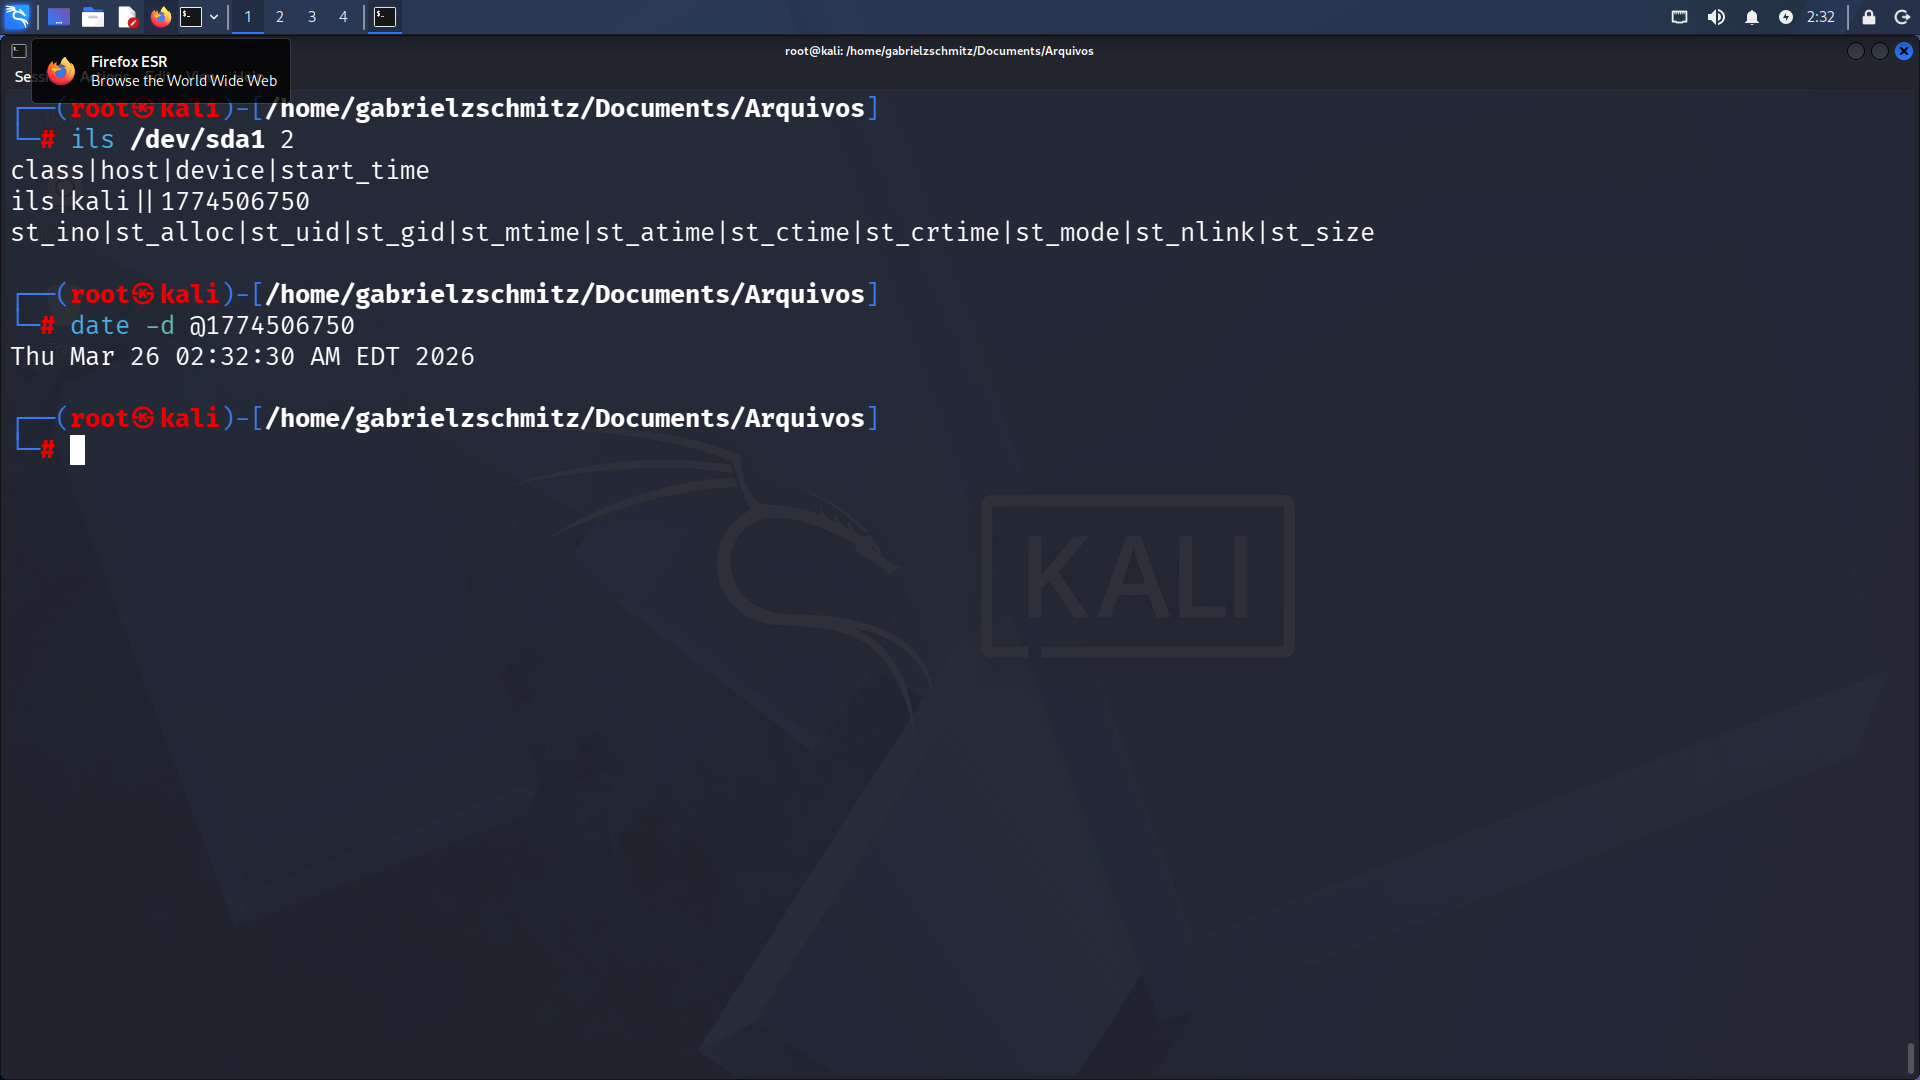
\includegraphics[width=0.99\textwidth]{./fig/fig12.9.png}
\caption{Resultado do comando ils aplicado à partição /dev/sda1}
\label{fig:fig12.9}
\end{figure}

\newpage

\question[Atividade 12.10]{Aquisição de imagem de disco no Kali Linux}

\begin{figure}[H]
\centering
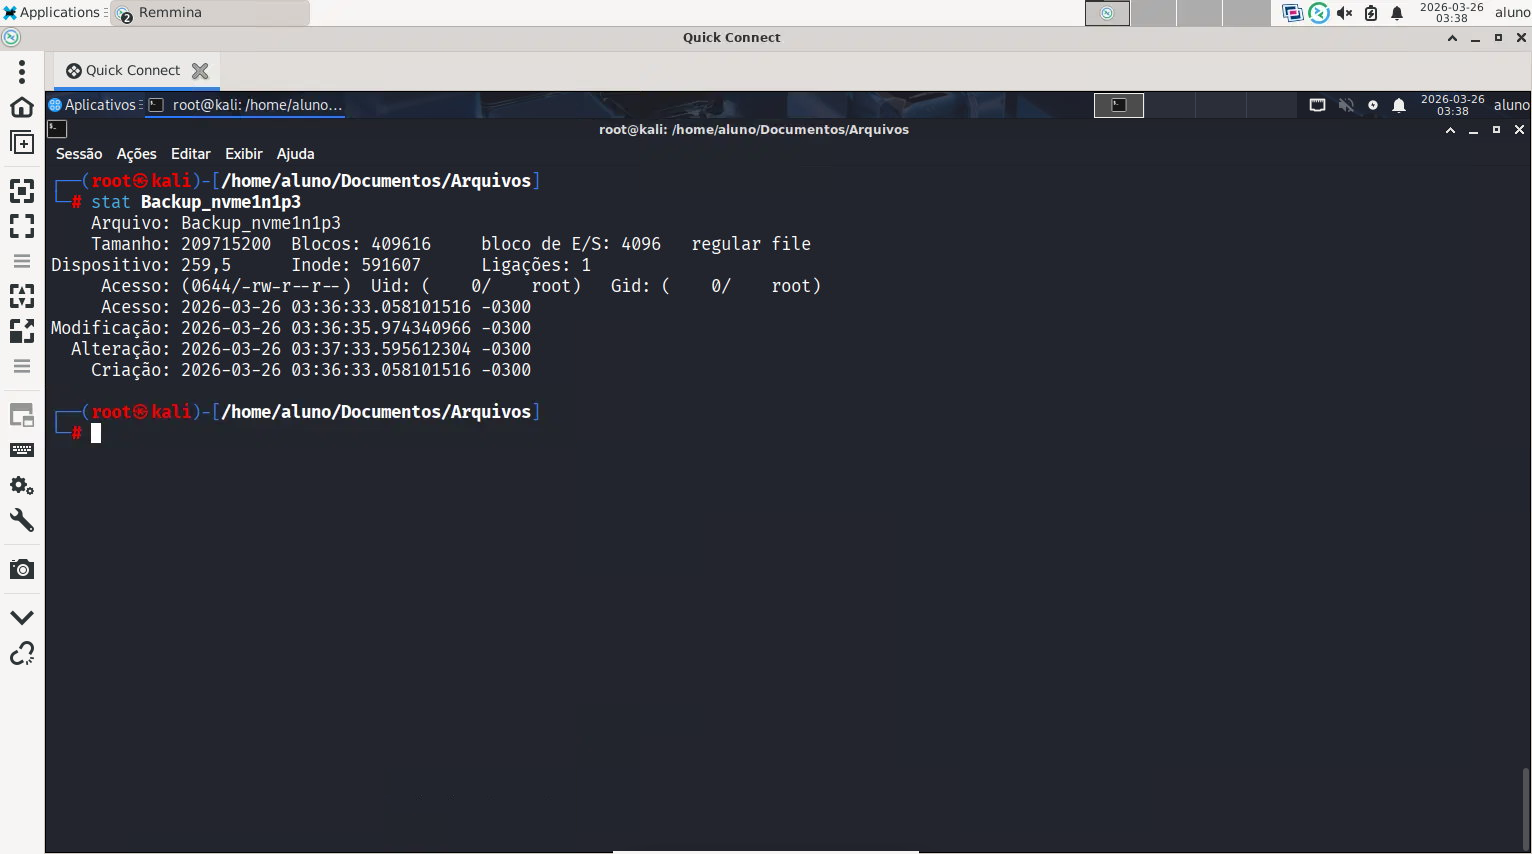
\includegraphics[width=0.99\textwidth]{./fig/fig12.10.png}
\caption{Informações do arquivo Backup\_nvme1n1p3 obtidas com stat}
\label{fig:fig12.10}
\end{figure}
